%\begin{figure*}[t]
%\centering
%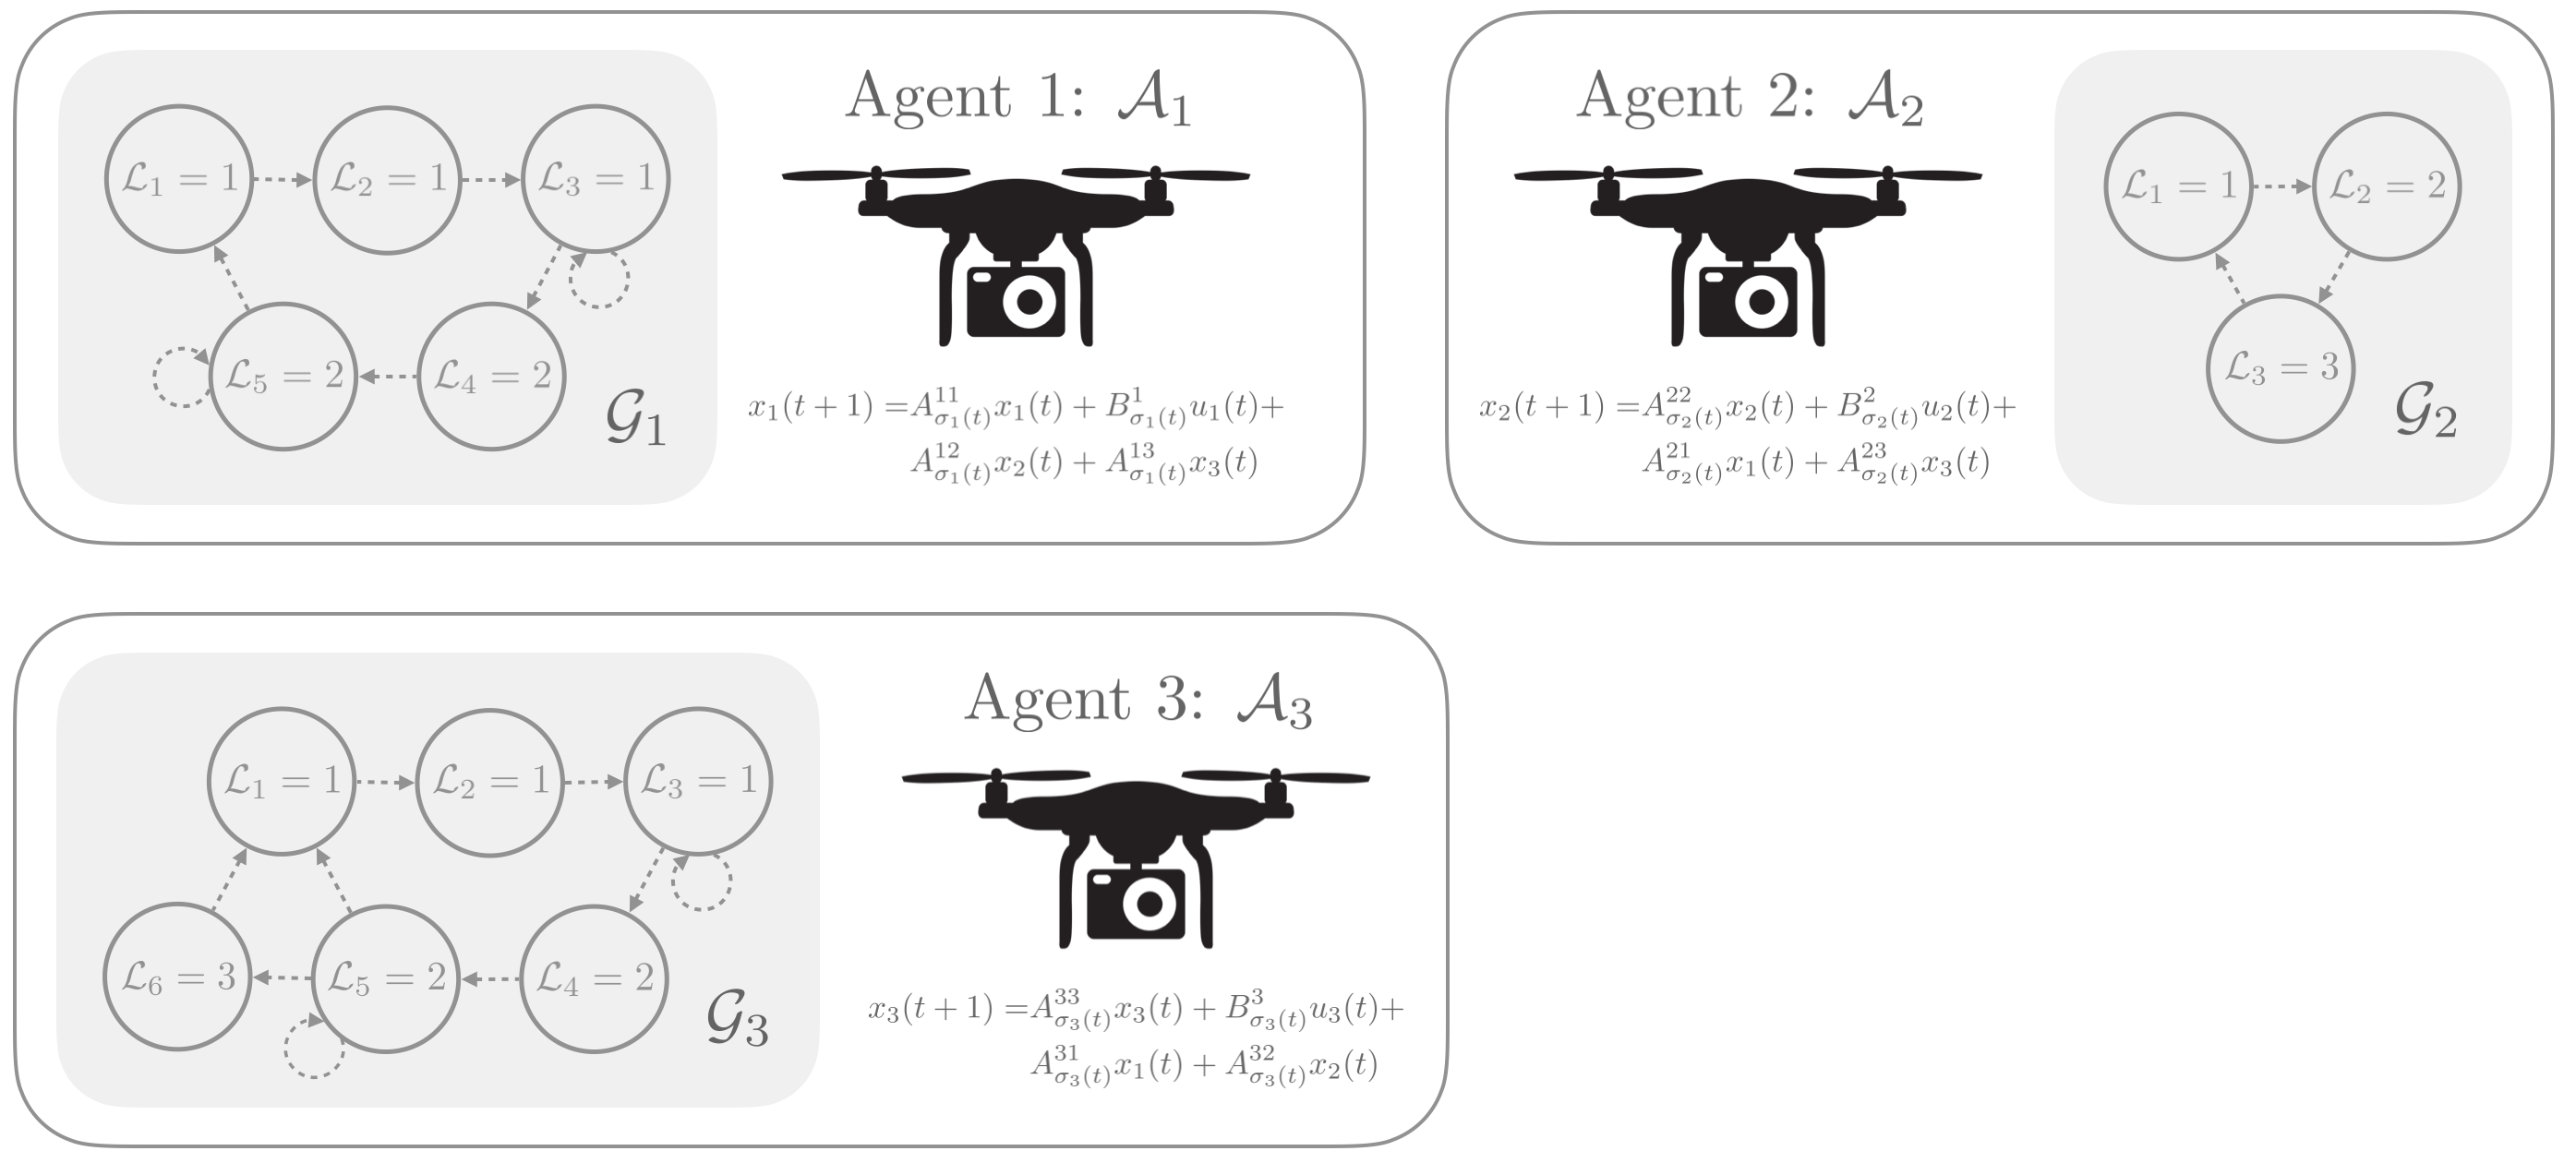
\includegraphics[width=\textwidth]{./figures/sample_system}
%\end{figure*}

\section{System Description}
Consider a collection of $\numagents\in\int\rgeq{1}$ external switching signals each respecting their own directed graph, $\ss_\agentidx(t)\in\Sigma(\graph_\agentidx)\ \agentidx\in\idxset{\numagents}$. Then the dynamics of the system being studied take the following form
\begin{align}
A(t)&=\begin{bmatrix}
A^{11}_{\ss_1(t)}&A^{12}_{\ss_1(t)}&\cdots&A^{1\numagents}_{\ss_1(t)},\\
A^{21}_{\ss_2(t)}&A^{22}_{\ss_2(t)}&\cdots&A^{2\numagents}_{\ss_2(t)},\\
\vdots&\vdots & \ddots & \vdots\\
A^{\numagents 1}_{\ss_\numagents(t)} & A^{\numagents 2}_{\ss_\numagents(t)} &\cdots & A^{\numagents \numagents}_{\ss_\numagents(t)} 
\end{bmatrix},\\
B(t)&=\begin{bmatrix}
B^{1}_{\ss_1(t)}&0&\cdots&0,\\
0&B^{2}_{\ss_2(t)}&\cdots&0,\\
\vdots&\vdots & \ddots & \vdots\\
0 & 0 &\cdots & B^{\numagents}_{\ss_\numagents(t)} 
\end{bmatrix}.
\end{align}
This structure is motivated by distributed systems with coupling in the system's states. Note how each block-row is governed by a single switching signal. This makes intuitive sense because local switching signals are more likely to effect how neighboring states impact the local agent rather then how local states will effect neighboring agents.

Our objective is to design safe-set collections for systems with the above structure. Recall that every element in a safe-set collection must be within the one-step preset of the elements indexed by the possible states of the switching signal after a single time step. The structure of the system under consideration makes this an especially challenging prospect for two reasons. First, the number of successor safe-sets grows exponentially when there are two or more independent switching signals. Second, systems that take this form would likely be in a relatively high dimension making set-operations exponentially more expensive. These two challenges suggest that previous, set-based techniques will struggle due to poor scaling in both the state dimension and the number of modes. These concerns will be addressed by splitting the system into block-rows and looking for safe-set collections for each separately. Once found, the collections can be merged into a large collection with all possible switching signal states represented.

\subsection{Block-row Dynamics}
Looking only at the block row indexed by $\agentidx$, the dynamics can be rewritten as 
\begin{align}\label{eq:block-row-dyn}
x_\agentidx(t+1)&=A^{\agentidx\agentidx}_{\ss_\agentidx(t)}x_\agentidx(t)+B^\agentidx_{\ss_\agentidx(t)}u_\agentidx(t)\nonumber\\&\quad+\sum_{\tilde\agentidx\in\idxset{\numagents}\setminus \agentidx}A^{\agentidx\tilde\agentidx}_{\ss_\agentidx(t)}x_{\tilde\agentidx}(t)\\
=A^{\agentidx}_{\ss_\agentidx(t)}&x_\agentidx(t)+B^\agentidx_{\ss_\agentidx(t)}u_\agentidx(t)+E^\agentidx_{\ss_\agentidx(t)}\left[x_{\tilde\agentidx}(t)\right]_{\tilde\agentidx\in\idxset{\numagents}\setminus \agentidx}.
\end{align}
These dynamics and constraints are collected into the following tuple defining agent $\agentidx$,
$$\agent{\agentidx}\triangleq\{\{A^{\agentidx}_{\modeidx},B^\agentidx_{\modeidx},E^\agentidx_{\modeidx},\xcon[\modeidx]^\agentidx,\ucon[\modeidx]^\agentidx\}_{\modeidx=1}^{\nummodes[\agentidx]},\graph^\agentidx\}.$$

This system only has a single switching signal explicitly appearing, $\ss_\agentidx(t)$, and resembles a locally switched system with additive disturbances. Previous, robust switched techniques, such as those developed in \cite{Lavaei2021}, may seem like possible solutions. However, these previous techniques rely on bounded additive disturbances and the bounds on $\left[x_{\tilde\agentidx}(t)\right]_{\tilde\agentidx\in\idxset{\numagents}\setminus \agentidx}$ are not obvious. The full state constraints, $x_{\tilde{\agentidx}}\in\xcon[\tilde{\agentidx}]$, could be used but this would lead to conservative results. Alternatively, the current safe-set containing $x_{\tilde{\agentidx}}$ could be used. This however, returns the system to the centralized problem with its associated drawbacks. Furthermore, if \autoref{eq:block-row-dyn} represents a distributed system, this level of communication may be undesirable. Balancing these considerations, this work bounds the neighboring states within the convex hull of the union of the neighbor's safe-set collection. This only requires acquiring a single set and only relies on the state of the local switching signal. 

The reader may have noticed that a circular dependency arose in the previous discussion -- the safe-set collection for agent $\agentidx$ depends on the safe-set collection for agent ${\tilde{\agentidx}}$ which depends on the safe-set collection for agent $\agentidx$. This problematic cycle is addressed in the algorithm development covered in the following section. 